\documentclass[a4paper, 12pt, margins=2cm]{homework}
\usepackage{tikz}

\usepackage{graphicx}
\usepackage{color}
\usepackage{transparent}
\usepackage{dsfont}
\usepackage{microtype}
\usepackage{mathrsfs}
\usepackage[ngerman]{babel}
\usepackage{csquotes}
\usepackage[T1]{fontenc}
\usepackage{lmodern}
\usepackage{wasysym}

\setlength{\parindent}{0pt}

\newcommand{\R}{\mathbb{R}}
\newcommand{\N}{\mathbb{N}}
\newcommand{\Z}{\mathbb{Z}}
\newcommand{\Q}{\mathbb{Q}}

\name{Tobias Eidelpes}
\course{Technische Grundlagen der Informatik}
\term{2015WS}
\hwnum{4}
\hwtype{Übungsblatt}
\problemtitle{Aufgabe}
\solutiontitle{Lösung}

\begin{document}
  \problemnumber{2}
  \begin{problem}
  \end{problem}
  \begin{solution}
    \hfill
    \begin{enumerate}[label=(\arabic*)]\itemsep0pt
      \item richtig
      \item richtig
      \item richtig
      \item falsch
      \item richtig
      \item richtig
      \item falsch
      \item falsch
      \item richtig
      \item richtig 
      \item falsch
      \item falsch
    \end{enumerate}
  \end{solution}

  \begin{problem}
  \end{problem}
  \begin{solution}\hfill
    \begin{center}
      \begin{tikzpicture}[scale=0.2]
        \tikzstyle{every node}+=[inner sep=0pt]
        \draw [black] (18.4,-19.1) circle (3);
        \draw (18.4,-19.1) node {$1$};
        \draw [black] (31.9,-19.1) circle (3);
        \draw (31.9,-19.1) node {$2$};
        \draw [black] (45.8,-19.1) circle (3);
        \draw (45.8,-19.1) node {$3$};
        \draw [black] (59,-19.1) circle (3);
        \draw (59,-19.1) node {$4$};
        \draw [black] (21.4,-19.1) -- (28.9,-19.1);
        \fill [black] (28.9,-19.1) -- (28.1,-18.6) -- (28.1,-19.6);
        \draw (25.15,-18.6) node [above] {$0/0$};
        \draw [black] (34.9,-19.1) -- (42.8,-19.1);
        \fill [black] (42.8,-19.1) -- (42,-18.6) -- (42,-19.6);
        \draw (38.85,-18.6) node [above] {$1/0$};
        \draw [black] (48.8,-19.1) -- (56,-19.1);
        \fill [black] (56,-19.1) -- (55.2,-18.6) -- (55.2,-19.6);
        \draw (52.4,-18.6) node [above] {$0/0$};
        \draw [black] (17.077,-16.42) arc (234:-54:2.25);
        \draw (18.4,-11.85) node [above] {$1/0$};
        \fill [black] (19.72,-16.42) -- (20.6,-16.07) -- (19.79,-15.48);
        \draw [black] (30.577,-16.42) arc (234:-54:2.25);
        \draw (31.9,-11.85) node [above] {$0/0$};
        \fill [black] (33.22,-16.42) -- (34.1,-16.07) -- (33.29,-15.48);
        \draw [black] (58.438,-22.021) arc (-23.90748:-156.09252:6.605);
        \fill [black] (46.36,-22.02) -- (46.23,-22.95) -- (47.14,-22.55);
        \draw (52.4,-26.45) node [below] {$1/1$};
        \draw [black] (43.812,-21.341) arc (-46.61505:-133.38495:17.05);
        \fill [black] (20.39,-21.34) -- (20.63,-22.25) -- (21.31,-21.53);
        \draw (32.1,-26.5) node [below] {$1/0$};
      \end{tikzpicture}
    \end{center}
  \end{solution}
\newpage
  \problemnumber{5}
  \begin{problem}
  \end{problem}
  \begin{solution} \hfill
    \begin{center}
      \begin{tabular}{l|c}
        XOR       & 15 \\
        Flip-Flop & 50 \\
        Setup     & 05  \\ \hline
        Summe     & 70
      \end{tabular}
    \end{center}
    \[\text{Maximale Taktfrequenz} = \frac{1}{70}\text{ ns} \approx 14.29 \text{ MHz} \]
    \begin{center}
      Maximale Taktfrequenz der Flip-Flops (10 MHz) wirkt beschränkend. \\
      $\Longrightarrow$ \textbf{Lösung: 10 MHz}
    \end{center}
  \end{solution}

  \begin{problem}
  \end{problem}
  \begin{solution} \hfill
    \begin{enumerate}[label=(\alph*)]\itemsep0pt
      \item Es handelt sich um ein Mealy-Schaltwerk. Die Ausgabe ist dann eins,
            wenn hintereinander die Eingaben eins bis drei in Binär erfolgt sind.
    \end{enumerate}
    \begin{center}
      \begin{tabular}{r|cccc|cccc|cccc|cccc}
        $e_1$   & 0     & 0     & 1     & 1     & 0     & 0     & 1     & 1     & 0     & 0     & 1     & 1     & 0     & 0     & 1     & 1     \\
        $e_0$   & 0     & 1     & 0     & 1     & 0     & 1     & 0     & 1     & 0     & 1     & 0     & 1     & 0     & 1     & 0     & 1     \\
        $Q_1$   & 0     & 0     & 0     & 0     & 0     & 0     & 0     & 0     & 1     & 1     & 1     & 1     & 1     & 1     & 1     & 1     \\
        $Q_0$   & 0     & 0     & 0     & 0     & 1     & 1     & 1     & 1     & 0     & 0     & 0     & 0     & 1     & 1     & 1     & 1     \\ \hline
        Zustand & $Z_0$ & $Z_1$ & $Z_0$ & $Z_0$ & $Z_0$ & $Z_0$ & $Z_2$ & $Z_0$ & $Z_0$ & $Z_0$ & $Z_0$ & $Z_3$ & $Z_0$ & $Z_0$ & $Z_0$ & $Z_0$ \\ \hline
        $Q'_1$  & 0     & 0     & 0     & 0     & 0     & 0     & 1     & 0     & 0     & 0     & 0     & 1     & 0     & 0     & 0     & 0     \\
        $Q'_0$  & 0     & 1     & 0     & 0     & 0     & 0     & 0     & 0     & 0     & 0     & 0     & 1     & 0     & 0     & 0     & 0     \\ \hline
        $a$     & 0     & 0     & 0     & 0     & 0     & 0     & 0     & 0     & 0     & 0     & 0     & 1     & 0     & 0     & 0     & 0     \\ \hline
        $J_1$   & 0     & 0     & 0     & 0     & 0     & 0     & 1     & 0     & 0     & 0     & 0     & 1     & 0     & 0     & 0     & 0     \\
        $K_1$   & 1     & 1     & 1     & 1     & 1     & 1     & 0     & 1     & 1     & 1     & 1     & 0     & 1     & 1     & 1     & 1     \\
        $J_0$   & 0     & 1     & 0     & 0     & 0     & 0     & 0     & 0     & 0     & 0     & 0     & 1     & 0     & 0     & 0     & 0     \\
        $K_0$   & 1     & 0     & 1     & 1     & 1     & 1     & 1     & 1     & 1     & 1     & 1     & 0     & 1     & 1     & 1     & 1    
        \end{tabular}
    \end{center}
  \end{solution}
\newpage
  \begin{problem}
  \end{problem}
  \begin{solution} \hfill
    \begin{center}
      \begin{tikzpicture}[scale=0.2]
        \tikzstyle{every node}+=[inner sep=0pt]
        \draw [black] (18.4,-19.1) circle (3);
        \draw (18.4,-19.1) node {$\frac{1}{000}$};
        \draw [black] (31.9,-19.1) circle (3);
        \draw (31.9,-19.1) node {$\frac{2}{001}$};
        \draw [black] (45.8,-19.1) circle (3);
        \draw (45.8,-19.1) node {$\frac{3}{011}$};
        \draw [black] (59.1,-19.1) circle (3);
        \draw (59.1,-19.1) node {$\frac{4}{111}$};
        \draw [black] (21.138,-17.889) arc (107.44657:72.55343:13.383);
        \fill [black] (29.16,-17.89) -- (28.55,-17.17) -- (28.25,-18.13);
        \draw (25.15,-16.77) node [above] {$01$};
        \draw [black] (34.652,-17.919) arc (107.17785:72.82215:14.215);
        \fill [black] (43.05,-17.92) -- (42.43,-17.21) -- (42.14,-18.16);
        \draw (38.85,-16.79) node [above] {$01$};
        \draw [black] (48.567,-17.955) arc (106.27603:73.72397:13.856);
        \fill [black] (56.33,-17.96) -- (55.71,-17.25) -- (55.43,-18.21);
        \draw (52.45,-16.9) node [above] {$01,11$};
        \draw [black] (17.077,-16.42) arc (234:-54:2.25);
        \draw (18.4,-11.85) node [above] {$10,00$};
        \fill [black] (19.72,-16.42) -- (20.6,-16.07) -- (19.79,-15.48);
        \draw [black] (30.577,-16.42) arc (234:-54:2.25);
        \draw (31.9,-11.85) node [above] {$00$};
        \fill [black] (33.22,-16.42) -- (34.1,-16.07) -- (33.29,-15.48);
        \draw [black] (56.518,-20.608) arc (-67.71817:-112.28183:10.729);
        \fill [black] (48.38,-20.61) -- (48.93,-21.37) -- (49.31,-20.45);
        \draw (52.45,-21.91) node [below] {$10$};
        \draw [black] (29.104,-20.174) arc (-74.72021:-105.27979:15.004);
        \fill [black] (21.2,-20.17) -- (21.84,-20.87) -- (22.1,-19.9);
        \draw (25.15,-21.2) node [below] {$10$};
        \draw [black] (43.137,-20.465) arc (-69.78811:-110.21189:12.408);
        \fill [black] (34.56,-20.47) -- (35.14,-21.21) -- (35.49,-20.27);
        \draw (38.85,-21.73) node [below] {$10$};
        \draw [black] (44.477,-16.42) arc (234:-54:2.25);
        \draw (45.8,-11.85) node [above] {$00$};
        \fill [black] (47.12,-16.42) -- (48,-16.07) -- (47.19,-15.48);
        \draw [black] (57.777,-16.42) arc (234:-54:2.25);
        \draw (59.1,-11.85) node [above] {$01,00$};
        \fill [black] (60.42,-16.42) -- (61.3,-16.07) -- (60.49,-15.48);
        \draw [black] (57.821,-21.811) arc (-29.18132:-150.81868:21.844);
        \fill [black] (57.82,-21.81) -- (56.99,-22.27) -- (57.87,-22.75);
        \draw (38.75,-33.5) node [below] {$11$};
        \draw [black] (57.253,-21.459) arc (-43.37106:-136.62894:16.169);
        \fill [black] (57.25,-21.46) -- (56.34,-21.7) -- (57.07,-22.38);
        \draw (45.5,-27.02) node [below] {$11$};
        \draw [black] (58.872,-22.089) arc (-8.58592:-171.41408:20.35);
        \fill [black] (18.63,-22.09) -- (18.25,-22.95) -- (19.24,-22.8);
        \draw (38.75,-39.9) node [below] {$11$};
      \end{tikzpicture}
    \end{center}

    \begin{enumerate}[label=(\alph*)]\itemsep0pt
      \item \hfill
      \begin{center}
        \begin{tabular}{cc|cc|cc}
          $e_1$ & $e_0$ & $Q_1$ & $Q_0$ & $D_1$ & $D_0$ \\ \hline
          0     & 0     & 0     & 0     & 0     & 0     \\
          0     & 0     & 0     & 1     & 0     & 1     \\
          0     & 0     & 1     & 0     & 1     & 0     \\
          0     & 0     & 1     & 1     & 1     & 1     \\
          0     & 1     & 0     & 0     & 0     & 1     \\
          0     & 1     & 0     & 1     & 1     & 0     \\
          0     & 1     & 1     & 0     & 1     & 1     \\
          0     & 1     & 1     & 1     & 1     & 1     \\
          1     & 0     & 0     & 0     & 0     & 0     \\
          1     & 0     & 0     & 1     & 0     & 0     \\
          1     & 0     & 1     & 0     & 1     & 1     \\
          1     & 0     & 1     & 1     & 1     & 1     \\
          1     & 1     & 0     & 0     & 1     & 1     \\
          1     & 1     & 0     & 1     & 1     & 1     \\
          1     & 1     & 1     & 0     & 1     & 1     \\
          1     & 1     & 1     & 1     & 0     & 0    
        \end{tabular}
      \end{center}
    \item \hfill

    \begin{minipage}{0.5\textwidth}
      \begin{center}
        \begin{tabular}{cccccc}
                                          & $\neg Q_0$             & $Q_0$                  & $Q_0$                  & $\neg Q_0$             &            \\ \cline{2-5}
          \multicolumn{1}{c|}{$\neg Q_1$} & \multicolumn{1}{c|}{1} & \multicolumn{1}{c|}{1} & \multicolumn{1}{c|}{1} & \multicolumn{1}{c|}{1} & $e_0$      \\ \cline{2-5}
          \multicolumn{1}{c|}{$Q_1$}      & \multicolumn{1}{c|}{0} & \multicolumn{1}{c|}{0} & \multicolumn{1}{c|}{0} & \multicolumn{1}{c|}{0} & $e_0$      \\ \cline{2-5}
          \multicolumn{1}{c|}{$Q_1$}      & \multicolumn{1}{c|}{1} & \multicolumn{1}{c|}{0} & \multicolumn{1}{c|}{1} & \multicolumn{1}{c|}{1} & $\neg e_0$ \\ \cline{2-5}
          \multicolumn{1}{c|}{$\neg Q_1$} & \multicolumn{1}{c|}{1} & \multicolumn{1}{c|}{1} & \multicolumn{1}{c|}{1} & \multicolumn{1}{c|}{0} & $\neg e_0$ \\ \cline{2-5}
                                          & $e_1$                  & $e_1$                  & $\neg e_1$             & $\neg e_1$             &           
        \end{tabular}
        \begin{align*}
          D_1:\quad & (e_0 \wedge \neg Q_1) \vee \\
                    & (\neg e_1 \wedge \neg e_0 \wedge Q_1) \vee \\
                    & (e_1 \wedge \neg e_0 \wedge \neg Q_1) \vee \\
                    & (\neg e_0 \wedge \neg Q_1 \wedge Q_0) \vee \\
                    & (e_1 \wedge \neg e_0 \wedge Q_1 \wedge \neg Q_0)
        \end{align*}
      \end{center}
    \end{minipage}
    \begin{minipage}{0.5\textwidth}
      \begin{center}
        \begin{tabular}{cccccc}
                                          & $\neg Q_0$             & $Q_0$                  & $Q_0$                  & $\neg Q_0$             &            \\ \cline{2-5}
          \multicolumn{1}{c|}{$\neg Q_1$} & \multicolumn{1}{c|}{1} & \multicolumn{1}{c|}{0} & \multicolumn{1}{c|}{1} & \multicolumn{1}{c|}{1} & $e_0$      \\ \cline{2-5}
          \multicolumn{1}{c|}{$Q_1$}      & \multicolumn{1}{c|}{1} & \multicolumn{1}{c|}{0} & \multicolumn{1}{c|}{0} & \multicolumn{1}{c|}{0} & $e_0$      \\ \cline{2-5}
          \multicolumn{1}{c|}{$Q_1$}      & \multicolumn{1}{c|}{0} & \multicolumn{1}{c|}{1} & \multicolumn{1}{c|}{1} & \multicolumn{1}{c|}{1} & $\neg e_0$ \\ \cline{2-5}
          \multicolumn{1}{c|}{$\neg Q_1$} & \multicolumn{1}{c|}{1} & \multicolumn{1}{c|}{1} & \multicolumn{1}{c|}{1} & \multicolumn{1}{c|}{0} & $\neg e_0$ \\ \cline{2-5}
                                          & $e_1$                  & $e_1$                  & $\neg e_1$             & $\neg e_1$             &           
        \end{tabular}
        \begin{align*}
          D_0:\quad & (\neg e_0 \wedge Q_0) \vee \\
                    & (e_1 \wedge \neg e_0 \wedge \neg Q_1) \vee \\
                    & (\neg e_1 \wedge \neg e_0 \wedge \neg Q_1) \vee \\
                    & (\neg e_1 \wedge e_0 \wedge \neg Q_1) \vee \\
                    & (e_1 \wedge e_0 \wedge \neg Q_0)
        \end{align*}
      \end{center}
    \end{minipage}
\newpage
    \item \hfill

    \centering
    \def\svgwidth{1\textwidth}
    \input{Bsp7c.pdf_tex}
    \end{enumerate}
  \end{solution}
\newpage
  \begin{problem}
  \end{problem}
  \begin{solution} \hfill

    \begin{center}
      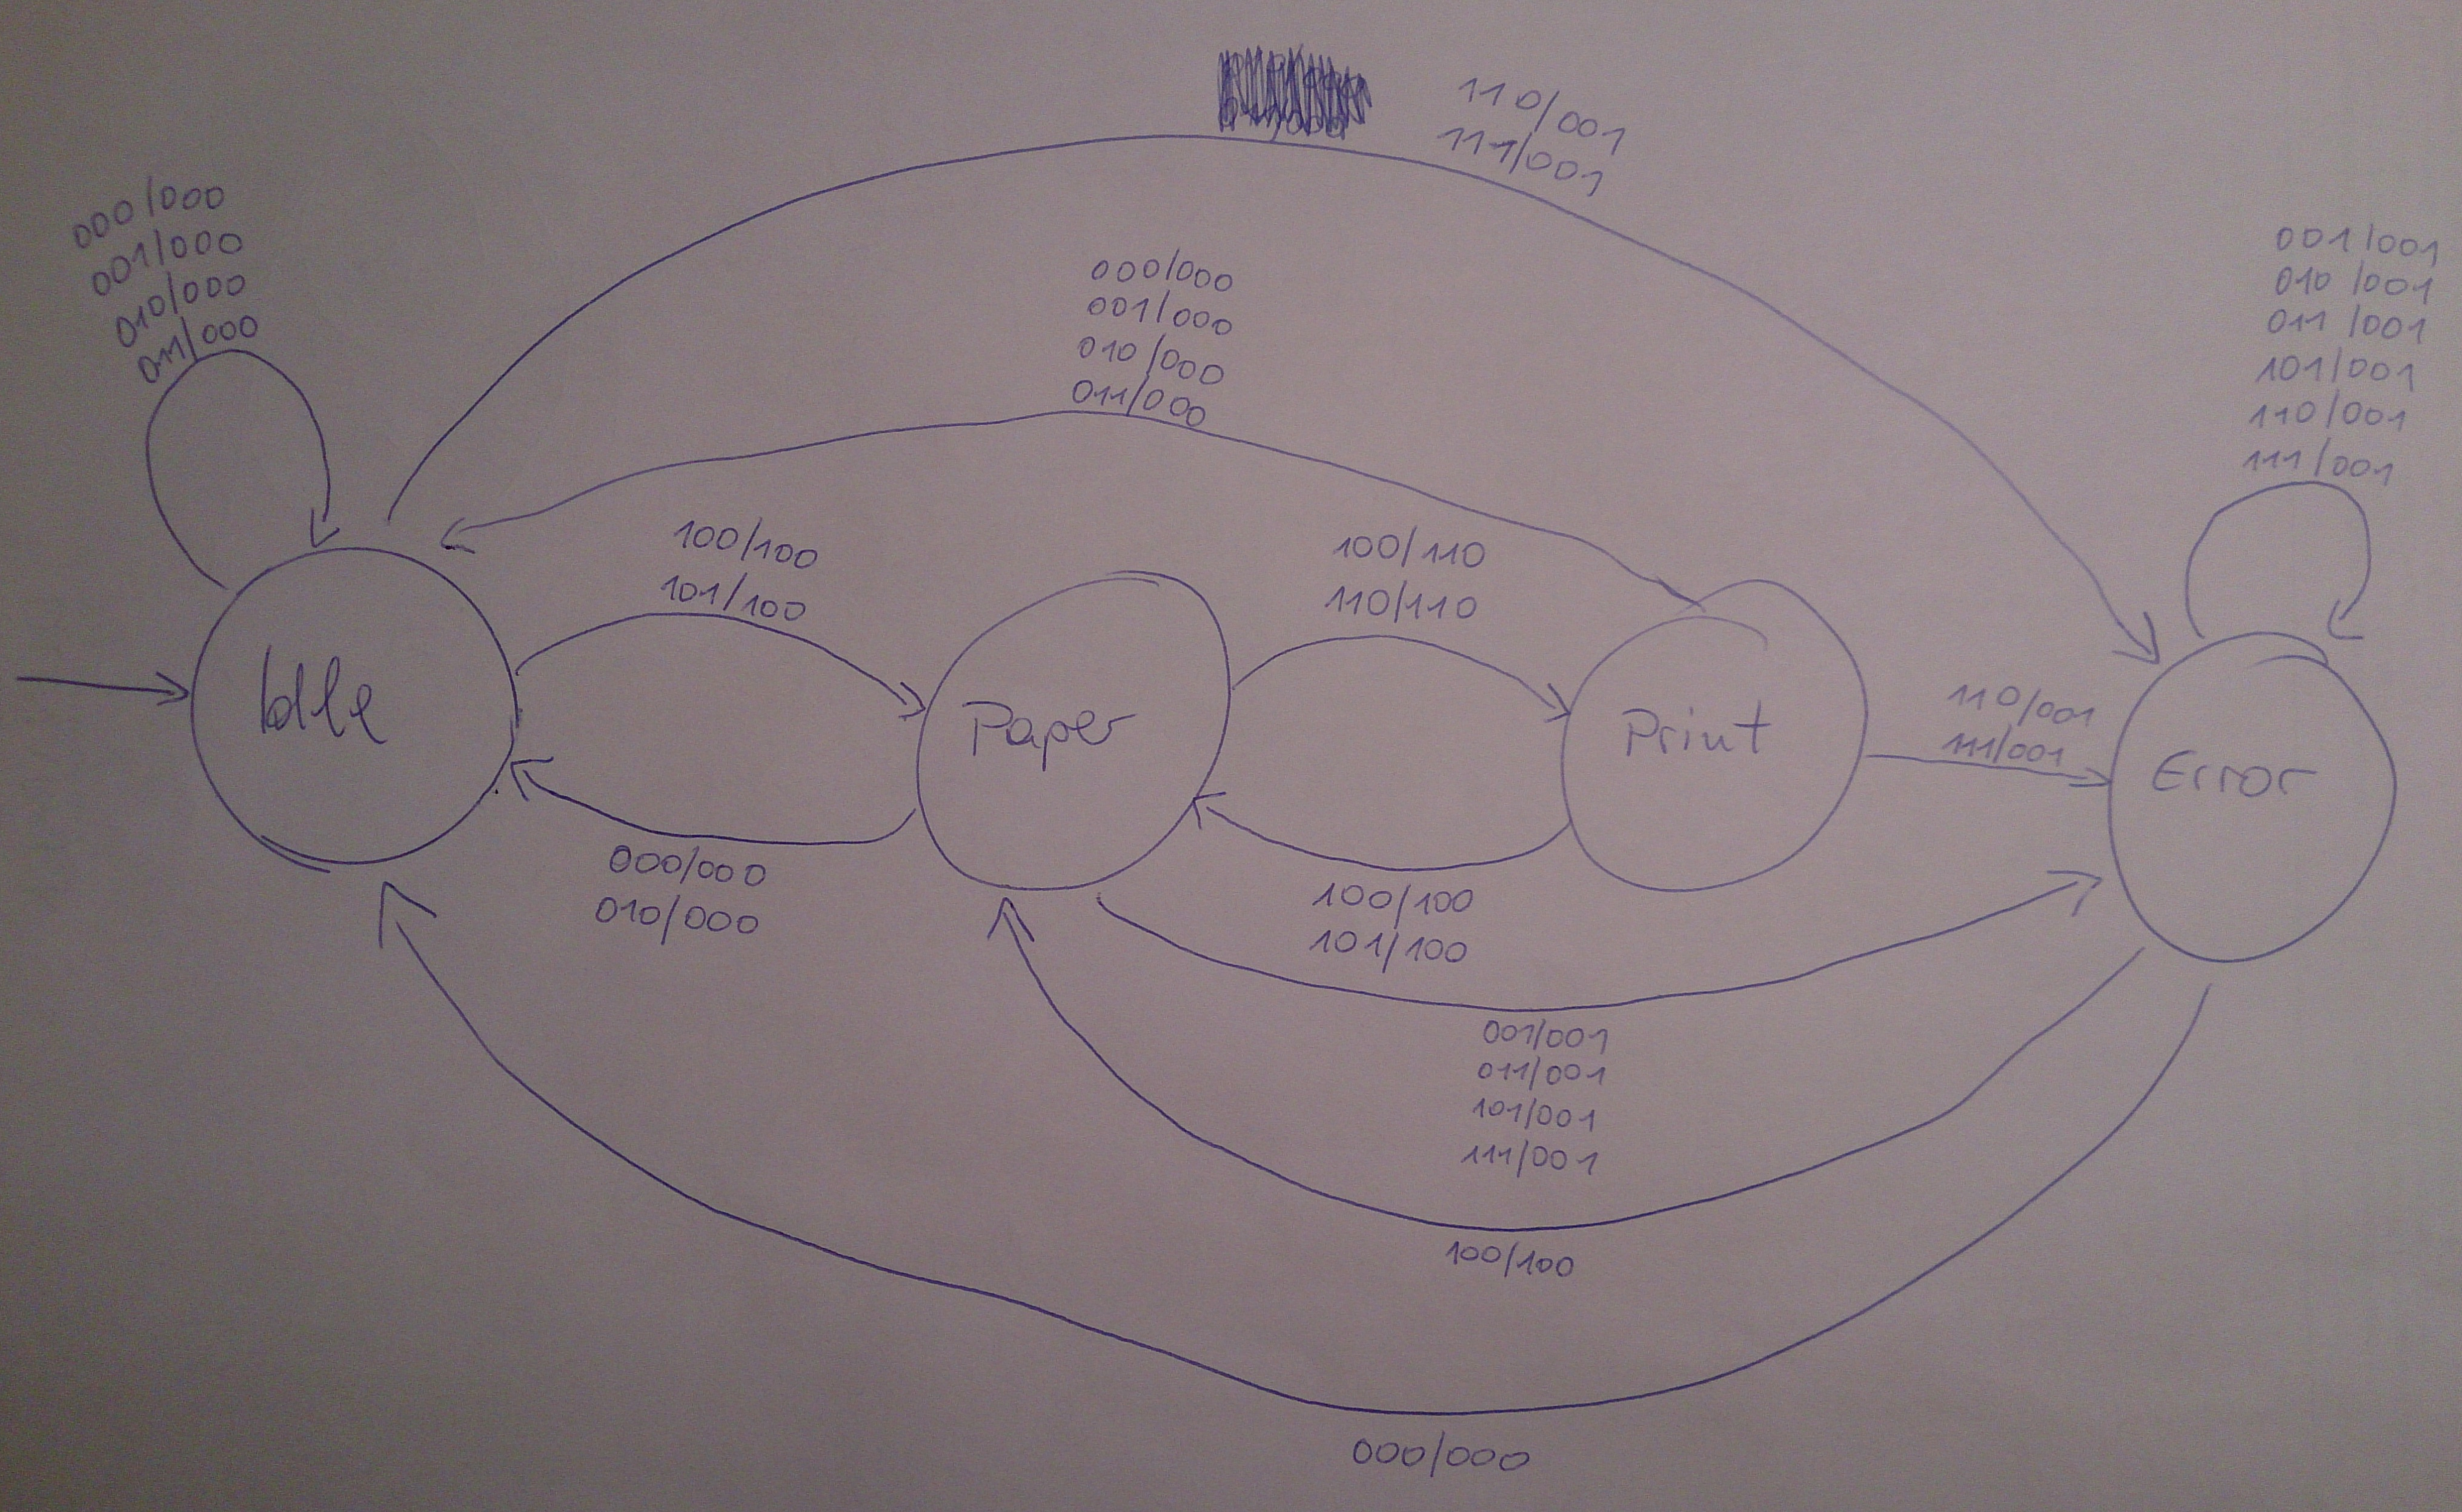
\includegraphics[scale=0.15, angle=-90]{Aufgabe8.jpg}
    \end{center}
  \end{solution}
\end{document}